%%%%%%%%%%%%%%%%%%%%%%%%%%%%%%%%%%%%%%%%%%%%%%%%%%%%%%%%%%%%%%%%%%%%%%%%%%%%%
%	E-Yantra, IIT-Bombay

%	Document Author: Bhumika Varshney
%	Date: 30th June,2015

%%%%%%%%%%%%%%%%%%%%%%%%%%%%%%%%%%%%%%%%%%%%%%%%%%%%%%%%%%%%%%%%%%%%%%%%%%%%%

\documentclass[10pt,red]{beamer} 
% change the alerted colour to blue
\setbeamercolor{alerted text}{fg=blue}

\usetheme{berlin}
% theme split
\usepackage{beamerthemesplit}

% theme shadow
\usepackage{beamerthemeshadow}

% For including figures
\usepackage{graphicx}

% logo
\logo{
\includegraphics[height=1cm]{iitblogo.pdf}}


% sf family, bold font
\sffamily \bfseries
% Beginning of title page
\title
% content inside [] appears at bottom of all page. content inside {} appears on first page as title. double backslash means line change 
[
	Firebird LPC2148 Robotics Research Platform	% bottom
	\hspace{0.5cm}
	\insertframenumber/\inserttotalframenumber
]
{
	LCD Interfacing on Firebird V Robot
}

\author
[
	www.e-yantra.org
]
{
	e-Yantra Team \\[20pt]
  Embedded Real-Time Systems Lab\\
  Indian Institute of Technology-Bombay \\
}
\date
{
IIT Bombay \\ {\today}
}
 
 
\begin{document}  

%Slide-1 for title page
\begin{frame}
   \titlepage
\end{frame}

%Slide-2 Content & Agenda for Talk 
\section*{outline}
\begin{frame}
	\frametitle{Agenda for Discussion}
	\tableofcontents
\end{frame}

\section{Introduction}
\subsection{LCD-Definition}
\begin{frame}
	\frametitle{Liquid Crystal Display} \pause
	\begin{enumerate}
		\item<+-|alert@+> A liquid crystal display (LCD) is a thin, flat panel used for electronically displaying information such as text, images, and moving pictures \\[10pt]
		
		\item<+-|alert@+> LCDs are economical and easy to use device. These are most commonly used display devices in an embedded system. Commonly available display are set up as 16 to 20 characters by 1 to 4 lines \\[15pt] 
		\end{enumerate} 
		\pause
		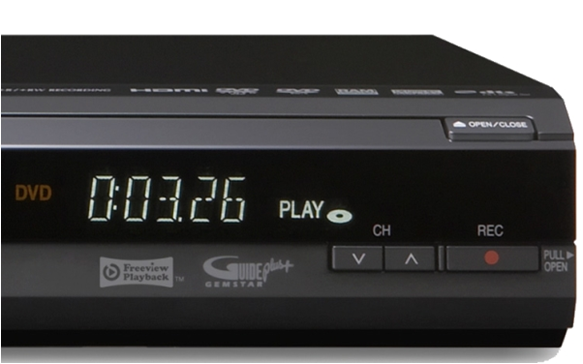
\includegraphics[width=0.2\linewidth]{example_1} 
		\hspace{1.5cm}
		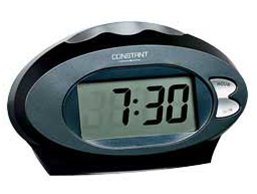
\includegraphics[width=0.2\linewidth]{example_2}
		\hspace{1.5cm}
		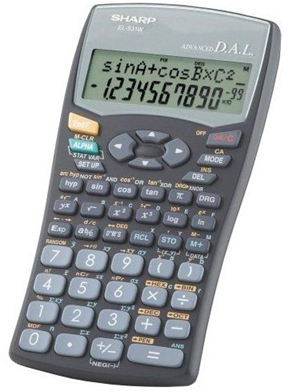
\includegraphics[width=0.2\linewidth]{example_3}
	
\end{frame}

\begin{frame}
	\frametitle{Dot Matrix Liquid Crystal Display} \pause
	\begin{enumerate}
	\item<+-|alert@+> LCD used here has HD44780 dot matrix lcd controller. It is also called 16x2 Alpha Numeric LCD \\[10pt]
	\item<+-|alert@+> It can be configured to drive a dot-matrix liquid crystal display under the control of a 4 or 8-bit	microprocessor \\[15pt]
	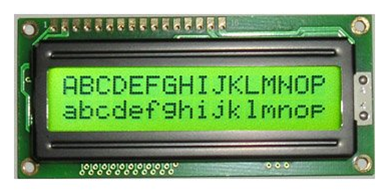
\includegraphics[width=0.8\linewidth]{lcd_display}
	\end{enumerate}
\end{frame}

\section{Understanding LCD}
\subsection{Pin-Configuration}
\begin{frame}
	\hspace{1.5cm}\frametitle{Pin-Configuration} \pause
	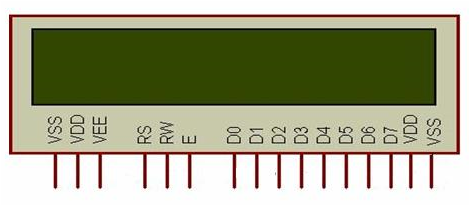
\includegraphics[width=0.5\linewidth]{pin_configuration} \pause
	
	\begin{tabular}{|c|c|}
				\noalign{\hrule height 0.5pt}
				Pin & Description  \pause \\  
				\noalign{\hrule height 1pt} 
				\vspace{2pt} 
				Vss & Ground \pause \\
				\hline 
				\vspace{2pt}
				Vdd & Supply Voltage \pause \\
				\hline 
				\vspace{2pt} 
				Vee & Contrast Voltage \pause \\
				\hline 
				\vspace{2pt} 
				RS & Register Select \pause \\
				\hline 
				\vspace{2pt} 
				RW & Read/Write \pause \\
				\hline 
				\vspace{2pt} 
				E & Enable \pause \\
				\hline 
				\vspace{2pt} 
				D0-D7 & Bidirectional Data Bus \pause \\
				\hline 
				\vspace{2pt} 
				Vdd,Vss & Back Light Supply  \pause \\
				\noalign{\hrule height 0.5pt}			
	\end{tabular}
\end{frame}
	
\subsection{Control Pins}
	\begin{frame}
		\frametitle{Control Pins} \pause
			\begin{enumerate}
				\item <+-|alert@+> Register Select
				\begin{itemize}
					\item <+-|alert@+> If \color{red!80}RS=0\color{black} ; Command Register
					\item <+-|alert@+> If \color{red!80}RS=1\color{black} ; Data Register
				\end{itemize}
				\item <+-|alert@+> Read/Write Select
				\begin{itemize}
					\item <+-|alert@+> If \color{red!80}RW=0\color{black} ; Write Mode
					\item <+-|alert@+> If \color{red!80}RW=1\color{black} ; Read Mode
				\end{itemize}
				\item <+-|alert@+> Enable
				\begin{itemize}
					\item <+-|alert@+> Used to latch the data present on the data pins
					\item <+-|alert@+> A high-to-low edge is needed to latch the data
				\end{itemize}
			\end{enumerate}
	\end{frame}
	
\subsection{Data Pins}
\begin{frame}
		\frametitle{Data Pins} \pause
			\begin{enumerate}[$\checkmark$]
			\item <+-|alert@+> Data Lines
				\begin{itemize}
					\item <+-|alert@+> There are 8 data pins from D0 to D7  \\[8pt]
					\item <+-|alert@+> Bidirectional Data / Command Pins \\[8pt]
					\item <+-|alert@+> Alpha Numeric Character  are sent in ASCII format \\[8pt]
					\item <+-|alert@+> We can use LCD either 8 bit mode or 4 bit mode \\[8pt]
					\item <+-|alert@+> We use 4 bit mode: only D4 to D7 data pins are used  \\[8pt]	
				\end{itemize}
			\end{enumerate}
	\end{frame}

\section{LCD Programming}
\subsection{LCD Interfacing}
\begin{frame}
		\frametitle{LCD Interfacing} \pause
		\hspace{1.5cm}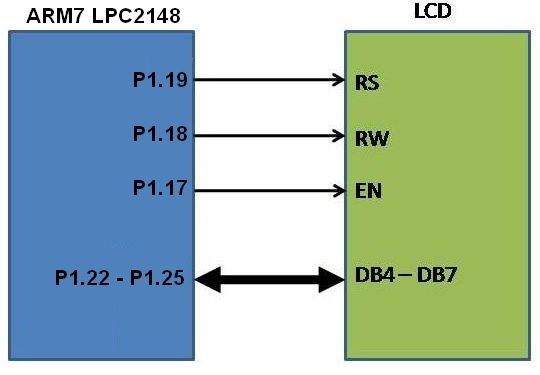
\includegraphics[scale=0.60]{lcd_interfacing}
\end{frame}
		
\subsection{Some Important commands}
\begin{frame}
		\frametitle{Some Important Commands} \pause
		\begin{tabular}{|c|c|}
				\noalign{\hrule height 0.5pt}
				Description & Hex  \pause \\  
				\noalign{\hrule height 1pt} 
				\vspace{2pt} 
				Function set (8-bit interface, 2 lines, 5*7 Pixels) & 38 \pause \\
				\hline 
				\vspace{2pt}
				Function set (4-bit interface, 2 lines, 5*7 Pixels) & 28 \pause \\
				\hline 
				\vspace{2pt} 
				Clear display screen & 01 \pause \\
				\hline 
				\vspace{2pt} 
				Return Home (First line first block) & 02 \pause \\
				\hline 
				\vspace{2pt} 
				Display ON cursor Blinking & 0F \pause \\
				\hline 
				\vspace{2pt} 
				Address for Line 1 & 80 \pause \\
				\hline 
				\vspace{2pt} 
				Address for Line 2 & C0 \pause \\
				\hline 
				\vspace{2pt} 
				Display ON cursor OFF & 0C  \pause \\
				\noalign{\hrule height 0.5pt}			
	\end{tabular}
\end{frame}	

\subsection{LCD Initialization}
\begin{frame}
	\frametitle{Steps for LCD Initialization} \pause
	\begin{enumerate}
		\item <+-|alert@+> Set Port1 as GPIO Port \\[8pt]
		\item <+-|alert@+> Initialize Port1 as Output Port \\[8pt]
		\item <+-|alert@+> Set  Control Lines   i.e.	RS=0 and RW=0 \\[8pt]
		\item <+-|alert@+> Send LCD init value i.e. 0x38 for 8-bit mode OR 0x28 for 4-bit mode \\[8pt]
		\item <+-|alert@+> Generate High-Low Pulse on Enable Pin of LCD \\[8pt]
		\item <+-|alert@+> Send LCD Clear value i.e. 0x01 \\[8pt]
		\item <+-|alert@+> Send LCD Display On value i.e. 0x0F \\[8pt]
		\item <+-|alert@+> Send LCD Cursor Home i.e. 0x02	\\[8pt]
	\end{enumerate}
\end{frame}

\subsection{Programming}
\begin{frame}[shrink = 2,fragile] 
	\frametitle{Syntax for C-Program}\pause
	
		\begin{block}<1->{\#include}\pause
		\begin{semiverbatim}
				#include <lpc214x.h>
				#include "LCD.h"                // User-defined header file
 		\end{semiverbatim}
		\end{block} \pause
		
	\begin{block}<2->{Main Program}\pause
		\begin{semiverbatim}
				int main (void) 
				\{
			\ \    Init_LCD_Pin();
			\ \    LCD_Init();
			\ \    LCD_Clear();
			\ \    LCD_Cursor(1,1);
			\ \    LCD_String("E-yantra");
			\ \    LCD_Cursor(2,3);
			\ \    LCD_String("IIT-Bombay");
			\ \	   while(1);	
				\}	
 		\end{semiverbatim}
		\end{block}	
\end{frame}

\begin{frame}[shrink=0,fragile]
	\frametitle{LCD.h- The Header File} \pause
		  \begin{enumerate}
		    \item <+-|alert@+> This file must be copied into Project Folder  \pause \\[10pt]
		  \end{enumerate}	
		%\begin{block}<1->{Look inside LCD.h}	\pause
		   \begin{semiverbatim}
\color{green!80} //define port where LCD is connected \color{black}
void Init_LCD_Pin();   \pause

\color{green!80} //LCD Initialization \color{black}
void LCD_Init();       \pause

\color{green!80} //To Send Command \color{black}
void LCD_Command(unsigned int data);   \pause

\color{green!80} //To write single character \color{black}
void LCD_Data(unsigned int data);	  \pause

\color{green!80} //To print string of characters \color{black}
void LCD_String(char*); 	  \pause 

\color{green!80}//To Place cursor at desired location \color{black}
void LCD_Cursor(char row,char column); \pause

\color{green!80} //To Print Numeric Value \color{black}
void LCD_Print(char row,char coloumn,unsigned int value,int digits);  \pause  
               
               
               
		   \end{semiverbatim}
		%\end{block} \pause
\end{frame}

\begin{frame}
\hskip4cm
\textbf{\LARGE Thank You!} \\[20pt]
\hskip3cm
\scriptsize Post your queries on: 
\hyperref[www.e-yantra.org]{\color{blue} http://qa.e-yantra.org/ \color{black}} 
\end{frame}
\end{document}

